%% MecHand manuscript — Journal of Cheminformatics (BMC / Springer Nature), Software article.
%% Class: Springer Nature LaTeX template (sn-jnl), which also covers BMC journals.
%% `make` downloads sn-jnl.cls and the .bst from
%% https://www.springernature.com/gp/authors/campaigns/latex-author-support
%% If you change the reference style option, update BST in the Makefile too.
%% Tables in analysis/results/ and figures/recognition-e2.pdf are generated by the
%% scripts in analysis/ (see analysis/README.md); do not edit them by hand.

\documentclass[pdflatex,lineno,sn-vancouver-num]{sn-jnl}

\usepackage[utf8]{inputenc}
\usepackage{amsmath,amssymb}
\usepackage{graphicx}
\usepackage{hyperref}
\usepackage{chemfig}          % the export example is compiled in the paper
\usepackage{tikz}
\usetikzlibrary{arrows.meta, bending, positioning, fit, calc}
\usepackage{booktabs}
\usepackage{tabularx}
\usepackage{xcolor}
% sn-jnl's own \orcid needs Orcidlogo.eps, which the template does not ship.
% sn-jnl also defines \orcidlogo, so clear it before orcidlink defines its own.
\let\orcidlogo\relax
\usepackage{orcidlink}

% Screenshots are shared with the project website.
\graphicspath{{../docs/public/img/}{figures/}}

\newcommand{\yes}{$\checkmark$}
\newcommand{\no}{--}

%% ─────────────────────────────────────────────────────────────────────────────
\begin{document}

\title[MecHand]{MecHand: freehand drawing of reaction mechanisms with in-browser
       handwriting recognition and direct export to \LaTeX{}}

%% \author* marks the corresponding author.
\author*[1,2,3]{\fnm{Jordi} \sur{Vill\`a-Freixa}\,\orcidlink{0000-0002-6359-3929}}\email{jordi.villa@uvic.cat}

\affil*[1]{\orgdiv{Department of Biosciences},
  \orgname{University of Vic -- Central University of Catalonia (UVic-UCC)},
  \orgaddress{\city{Vic}, \country{Spain}}}

\affil[2]{\orgname{IRIS-CC (Institut de Recerca i Innovaci\'o en Ci\`encies
  de la Vida i de la Salut a la Catalunya Central)},
  \orgaddress{\city{Vic}, \country{Spain}}}

\affil[3]{\orgdiv{Computational Biochemistry and Biophysics Lab, Research Group
  on Bioinformatics and Bioimaging (BI-SQUARE)},
  \orgname{Universitat de Vic -- Universitat Central de Catalunya (UVic-UCC)},
  \orgaddress{\city{Vic}, \country{Spain}}}

%% ── Abstract (≤ 350 words) ────────────────────────────────────────────────────
\abstract{%
Curved-arrow reaction mechanisms are central to how chemists reason, teach and
communicate, and they are still mostly drawn by hand. Turning such a sketch into a
figure for a manuscript means redrawing it in a structure editor, and optical
chemical structure recognition (OCSR) tools, which read molecules from images, do
not handle the electron-flow arrows that make a drawing a mechanism.
We present MecHand, an open-source web application that adds freehand mechanism
drawing to the Ketcher chemical editor. Structures, charges and curved arrows are
drawn with a stylus, a trackpad or a mouse. An online recogniser that runs entirely
in the browser reads the pen strokes, classifies atom labels with a point-cloud
gesture recogniser, anchors every curved arrow to an atom or a bond, checks the
electron bookkeeping, and inserts the result into Ketcher after the user confirms
it. Mechanisms are exported to TikZ and \texttt{chemfig} for \LaTeX{} and to CDXML
and MDL formats. On synthetic handwriting of thirteen textbook mechanisms from
organic, inorganic and biological chemistry, drawn in three hand styles, MecHand
recovers 87\,\% of the atoms, 85\,\% of the bonds and all curved and reaction arrows.
On the 126 drawings of the individual molecules it returns the exact structure for
65\,\% of them, against 40\,\% for DECIMER's model for hand-drawn images, with a
median recognition time of 0.1\,s. The application is tested automatically in the
Chromium, Firefox and WebKit browser engines, including a test that no data leaves
the browser.

\textbf{Scientific contribution:} MecHand is, to our knowledge, the first open-source
tool that recognises complete hand-drawn reaction mechanisms --- structures together
with their electron-flow arrows --- from pen strokes inside the web browser, checks
their electron flow and exports them directly to \LaTeX{}. It shows that online,
stroke-based recognition, with a small and openly extensible symbol model, can
outperform image-based recognition of hand-drawn molecules in an interactive
setting, while keeping every drawing on the user's computer.}

\keywords{reaction mechanism, curved arrows, electron flow, sketch recognition,
  handwriting recognition, chemical structure editor, Ketcher, \LaTeX, chemfig, TikZ}

\maketitle

%% ─────────────────────────────────────────────────────────────────────────────
\section{Background}
\label{sec:background}

The curved-arrow notation of reaction mechanisms is one of the most characteristic
languages of chemistry. Each arrow states where a pair of electrons (or, with a
half-headed ``fishhook'', a single electron) comes from and where it goes, and a
sequence of such arrows explains how bonds are broken and formed. Learning to draw
and read these arrows is a recognised difficulty for students
\cite{Bhattacharyya2005,Grove2012}, and mechanisms are therefore drawn constantly
--- on paper, on whiteboards and on tablets --- in teaching and research.

Turning a sketch into a figure for a paper, a thesis or lecture notes is, however,
still a manual task. Commercial structure editors such as ChemDraw and Marvin
provide mechanism arrows; Marvin~JS attaches its electron-flow arrows to lone
pairs, bonds and atoms and enforces rules on valid sources and targets
\cite{MarvinJS}. Open-source editors for the web, such as Ketcher
\cite{Karulin2011,Ketcher}, JSME \cite{Bienfait2013} and Kekule.js
\cite{Jiang2016}, are widely embedded in databases and teaching platforms. All of
them are operated with a mouse and toolbars, so the user has to translate what
they would draw by hand into a sequence of tool choices. In documents typeset with
\LaTeX{}, which is common in chemistry and physics, structures and arrows are
usually rewritten by hand in packages such as \texttt{chemfig} \cite{Tellechea2024}
or TikZ \cite{Tantau2015}, a slow and error-prone step.

Two lines of work address the gap between hand-drawn and digital chemistry.
\emph{Optical chemical structure recognition} (OCSR) reads structures from images
\cite{Rajan2020review}. Rule-based systems such as OSRA \cite{Filippov2009} were
followed by deep-learning models such as MolScribe \cite{Qian2023} and DECIMER
\cite{Rajan2023,Rajan2023ai}; DECIMER now includes a model trained for hand-drawn
structures \cite{Brinkhaus2024}. OCSR works on pixels after the drawing is
finished, recognises molecules rather than mechanisms, and requires a deep-learning
runtime, usually on a server; a benchmark for mechanistic images has only recently
been proposed \cite{Leung2024}. \emph{Online sketch recognition}, in contrast,
interprets the pen strokes as they are drawn. ChemInk \cite{Ouyang2011} showed that
this information --- stroke order, direction and shape --- allows accurate,
real-time recognition of hand-drawn molecules on a pen computer, but it handled
structures only and is not available as software.

Here we describe MecHand, which brings online recognition of complete mechanisms
to the browser. Its design goals were: (i)~structures, charges \emph{and}
electron-flow arrows are recognised together, as drawn on paper; (ii)~recognition
runs in the browser, with no installation, server or transfer of the user's
drawings; (iii)~the recognised mechanism lands in a full-featured, standard
chemical editor rather than in a separate format; (iv)~mechanisms can be exported
to \LaTeX{} as editable code; and (v)~the recogniser is transparent and its symbol
model can be extended by its users.

%% ─────────────────────────────────────────────────────────────────────────────
\section{Implementation}
\label{sec:implementation}

\subsection{Architecture}

MecHand is a single-page web application written in TypeScript with React and
built with Vite (Figure~\ref{fig:architecture}). Ketcher (version~3.18.0) is used
through its published npm packages, pinned to an exact version, rather than as a
fork; its standalone mode runs the Indigo toolkit \cite{Pavlov2011} compiled to
WebAssembly, so that chemistry operations such as layout, aromaticity and format
conversion happen in the browser. MecHand adds an ink layer over Ketcher's drawing
area, the online recogniser, a consolidation dialog, mechanism templates and
exporters. An optional server wraps DECIMER for users who want to compare the
in-browser recogniser with an image-based model.

\begin{figure}[t]
\centering
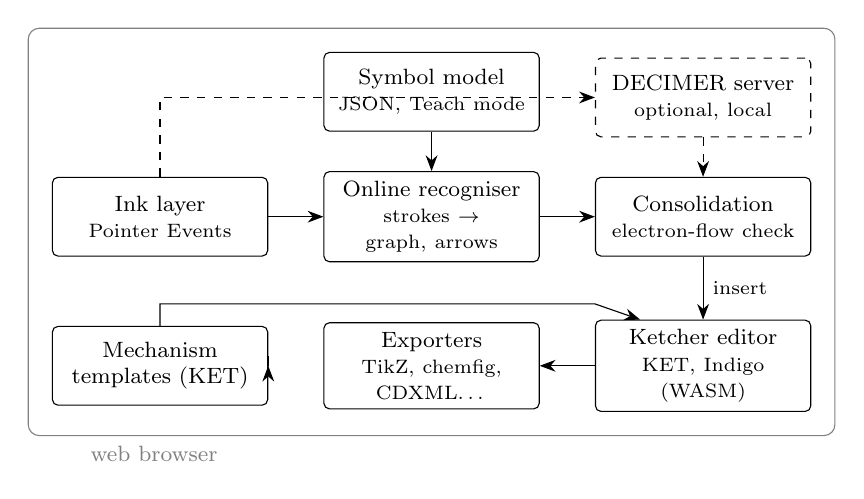
\begin{tikzpicture}[
  node distance=5mm and 7mm, >={Stealth[length=2mm]},
  box/.style={draw, rounded corners=2pt, align=center, font=\footnotesize,
              minimum height=10mm, text width=25mm, fill=white},
  opt/.style={box, dashed}]
  \node[box] (ink) {Ink layer\\\scriptsize Pointer Events};
  \node[box, right=of ink] (rec) {Online recogniser\\\scriptsize strokes $\rightarrow$ graph, arrows};
  \node[box, right=of rec] (dlg) {Consolidation\\\scriptsize electron-flow check};
  \node[box, below=8mm of dlg] (ket) {Ketcher editor\\\scriptsize KET, Indigo (WASM)};
  \node[box, left=of ket] (exp) {Exporters\\\scriptsize TikZ, chemfig, CDXML\ldots};
  \node[box, left=of exp] (tpl) {Mechanism\\templates (KET)};
  \node[box, above=5mm of rec] (model) {Symbol model\\\scriptsize JSON, Teach mode};
  \node[opt, above=5mm of dlg] (srv) {DECIMER server\\\scriptsize optional, local};
  \draw[->] (ink) -- (rec);
  \draw[->] (rec) -- (dlg);
  \draw[->] (dlg) -- node[right, font=\scriptsize] {insert} (ket);
  \draw[->] (ket) -- (exp);
  \draw[->] (tpl) -- (exp.west -| tpl.east) ;
  \draw[->] (tpl.north) |- ($(ket.north west)+(0,2mm)$) -- ($(ket.north)+(-8mm,0)$);
  \draw[->] (model) -- (rec);
  \draw[->, dashed] (ink.north) |- (srv.west);
  \draw[->, dashed] (srv) -- (dlg);
  \node[draw, gray, rounded corners=4pt, inner sep=3mm, fit=(ink)(rec)(dlg)(ket)(exp)(tpl)(model),
        label={[gray, font=\footnotesize]below left:web browser}] {};
\end{tikzpicture}
\caption{Architecture of MecHand. Everything inside the grey frame runs in the
  user's web browser; the DECIMER server (dashed) is optional and runs on the
  user's own computer.}
\label{fig:architecture}
\end{figure}

\subsection{Pen input}

Strokes are captured with the W3C Pointer Events API, which gives a single code
path for mouse, trackpad, touch and stylus. When the browser provides them,
coalesced events are used to obtain all samples between screen frames, which
matters for fast pen movements. Once a stylus has been used, touch input is
ignored for drawing (palm rejection), and the ink layer disables the browser's
touch gestures while freehand mode is on. Turning freehand mode off lets the
pointer through to Ketcher, so that hand drawing and Ketcher's tools can be
alternated at any time.

\subsection{Online recognition}
\label{sec:recognition}

The recogniser turns a list of strokes into a \emph{scene}: atoms (element, formal
charge, radical), bonds (order, wedges), curved arrows (start, end and signed bulge)
and reaction arrows and plus signs. It uses only geometry and a small symbol
classifier, so every decision can be inspected. All thresholds are expressed
relative to the drawn bond length $L$, which makes recognition independent of the
size of the drawing (Table~\ref{tab:parameters}).

\paragraph{Scale.} $L$ is estimated from two cues: the length of straight
stroke segments, and the height $h$ of strokes that are clearly letters (curly and
compact, such as C, O, S or B), using $L \approx h/0.38$. When there are few bonds
--- for example a Cl$_2$ molecule surrounded by labels --- straight letter strokes
(the stems of l, H or +) would otherwise bias the first cue, so the letter-based
estimate prevails unless both agree. Arrows are detected with a first estimate and
excluded before $L$ is refined, because a long reaction arrow would otherwise be
taken as a bond.

\paragraph{Arrows.} A stroke is an arrow if it ends with a head: either a sharp
reversal at its end, drawn without lifting the pen, or a separate small ``V'' (two
barbs) or single barb whose vertex lies at one end of the stroke and whose arms
point back along the shaft. The shaft must be at least $0.75\,L$ long and
\emph{smooth}: letters such as N or Z, or a zig-zag chain with a stroke next to its
end, have sharp corners that a curved arrow does not. Curved shafts become
electron-flow arrows --- a full head for an electron pair, a single barb for one
electron --- and long straight ones with a full head become reaction arrows. The
bulge of a curved arrow is the signed maximum distance of the shaft from its chord.

\paragraph{Letters and bonds.} The remaining strokes are split at their corners with
ShortStraw \cite{Wolin2008}, so that chains and rings may be drawn in one stroke.
Long straight pieces are bonds. Short strokes are letters when they cross another
short stroke (+, t), meet it in a T (H, F), meet it at an acute angle (N, M, Z;
bonds never meet at less than $60^\circ$), or stand upright beside a letter of the
same height (the l of Cl). Bonds stop short of an atom label in handwriting, and
these rules keep the bond that ends next to a letter separate from the letter.
Close, near-parallel lines are merged into double and triple bonds, and bond ends
closer than $0.32\,L$ are merged into atoms.

\paragraph{Atom labels and charges.} Letter strokes are grouped into labels and
split into characters, trying a few gap tolerances because letter spacing varies
between writers. Each character is classified with the \$P point-cloud recogniser
\cite{Vatavu2012}, which compares resampled clouds of 32 points and is therefore
independent of the number, order and direction of the strokes. A decoder then
chooses, among the best candidates of each character, the best \emph{chemically
valid} reading --- for instance ``Cl'' rather than ``CI'', ``Pt2$-$'' or ``O$-$''.
A label attaches to the nearest bond end, and absorbs every bond end within
$0.5\,L$, because the several bonds of a labelled centre (B in BF$_3$, a metal) need
not meet at one point. A charge sign attaches preferentially to the atom it is
written above and to the right of.

\paragraph{Electron flow.} Each end of a curved arrow is anchored to the nearest
atom or bond, as in Marvin~JS \cite{MarvinJS}. A simple checker then warns when an
electron-pair arrow starts at an atom without a lone pair, when an arrow starts or
ends on nothing, or when an arrow would give C, N, O or F more than an octet while
no bond to that atom is broken in the same step.

\begin{table}[t]
\caption{Main recognition parameters, relative to the drawn bond length $L$.}
\label{tab:parameters}
\begin{tabular}{@{}ll@{}}
\toprule
Parameter & Value \\
\midrule
Capital letter height & $0.38\,L$ (scale cue) \\
Minimum bond piece & $0.4\,L$ \\
Bond ends merged into one atom & within $0.32\,L$ \\
Double/triple bond: angle, separation & $<15^\circ$, $0.04$--$0.4\,L$ \\
Strokes grouped into one label & gap $<0.22\,L$ \\
Label attached to a bond end & within $0.6\,L$ \\
Charge attached to an atom & within $0.85\,L$ \\
Curved-arrow shaft & $\geq 0.75\,L$, no corner $>65^\circ$ \\
Reaction arrow & $\geq 1.2\,L$, straight, full head \\
\$P cloud size; augmented copies per glyph & 32 points; 6 \\
Character acceptance & score $\geq 0.6$ ($\geq 0.5$ with a margin of $0.1$) \\
\bottomrule
\end{tabular}
\end{table}

\subsection{The symbol model}

The ``model'' of the \$P classifier is data: a versioned JSON file of glyph
skeletons (letters for common elements, the digits 2--4 for charge magnitudes,
and $+$ and $-$, also circled), drawn as lines and arcs in a unit box. At start-up
each skeleton is expanded into copies with random slant, aspect ratio, rotation
and jitter, which gives about 600 templates and takes a fraction of a second. Two
further sources are added: samples contributed by users and kept in the
repository, and samples that each user records in the application's
\emph{Teach} mode. Teach samples are stored only in the browser's local storage and
contain just the symbol and the $(x,y)$ points of its strokes. A user can export
them and propose them for the shared model through a pull request; the model
version in use is shown in the application. Updating the model therefore requires
no retraining infrastructure: it is edited, tested and released like the code.

\subsection{Consolidation}

Recognition never changes the drawing silently. The user presses \emph{Recognize}
(or the space bar), and the ink is coloured by how each stroke was read --- bonds,
labels, arrows, or not understood --- while a dialog shows a clean rendering of the
result, a confidence estimate and any electron-flow warnings
(Figure~\ref{fig:interface}). The user then inserts the result into Ketcher, keeps
drawing to correct it, or discards the ink. The scene is passed to Ketcher in its
native KET format, with curved arrows as Ketcher's elliptical-arc arrows, so the
inserted mechanism is an ordinary, editable Ketcher drawing.

\begin{figure}[t]
\centering
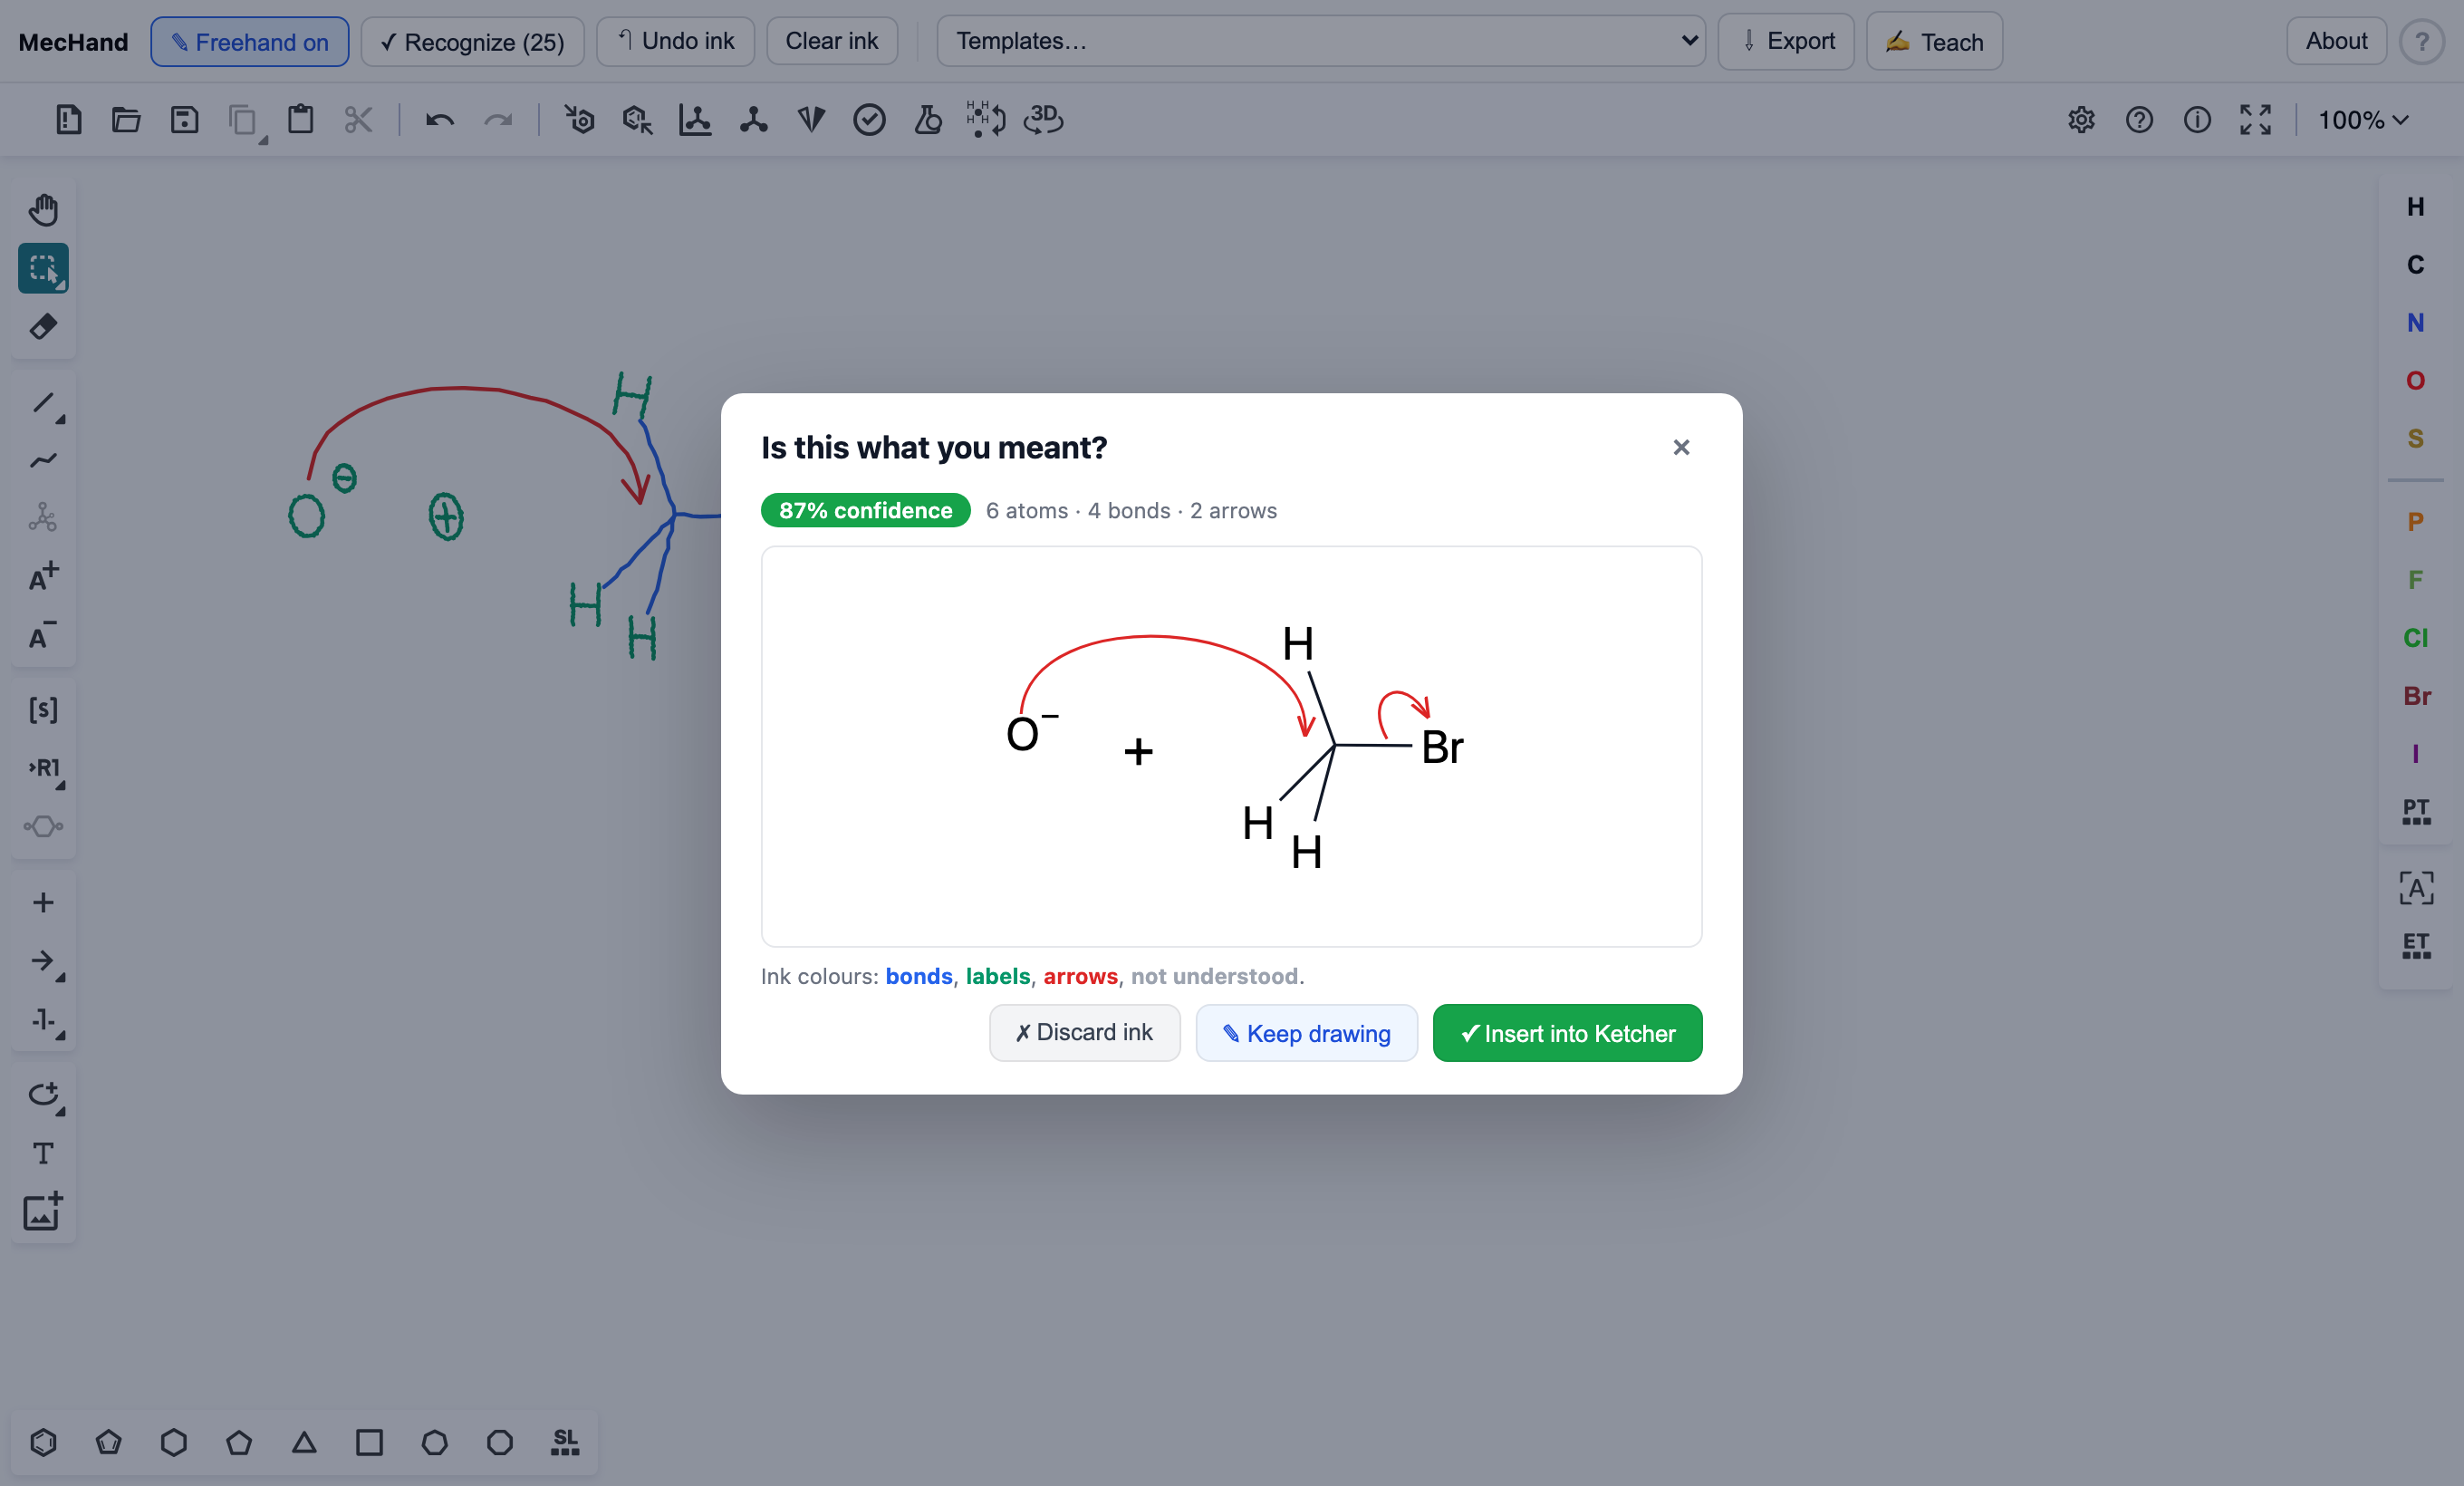
\includegraphics[width=\linewidth]{recognize-dialog.png}
\caption{The consolidation dialog. The S$_\mathrm{N}$2 reactants drawn by hand
  (left; ink coloured by interpretation) are shown as recognised, with the
  confidence and a summary, before they are inserted into Ketcher.}
\label{fig:interface}
\end{figure}

\subsection{Mechanism templates}

MecHand includes thirteen textbook mechanisms (Table~\ref{tab:benchmark}): six
organic (S$_\mathrm{N}$2, E2, nucleophilic addition to a carbonyl group, the first
step of aromatic nitration, a Diels--Alder reaction and the homolysis of Cl$_2$),
four inorganic (the NH$_3$--BF$_3$ Lewis adduct, associative substitution at
square-planar Pt(II), the hydrolysis of SiCl$_4$ and the Br{\o}nsted acidity of
[Fe(OH$_2$)$_6$]$^{3+}$) and three biochemical (acylation by a serine protease,
hydride transfer by alcohol dehydrogenase and phosphoryl transfer by a kinase).
They are generated reproducibly with RDKit \cite{RDKit} by a script that also checks
that atoms and formal charges balance across every reaction arrow and that every
arrow end resolves to the intended atom or bond. They serve as teaching material,
as test data for the recogniser and as test cases for the exporters.

\subsection{Export}

The exporters work on the Ketcher canvas, so they include anything drawn by hand
or with Ketcher's tools. The TikZ exporter writes absolute coordinates: atoms with
labels become nodes, bonds are drawn between node anchors so that they stop at the
labels, wedges become filled or hashed triangles, and Ketcher's elliptical-arc
arrows become cubic B\'ezier curves. For an arrow from $\mathbf{s}$ to $\mathbf{e}$
with bulge $h$ along the unit normal $\mathbf{n}$, the control points
\begin{equation}
  \mathbf{c}_1 = \mathbf{s} + \tfrac{4}{3}\,h\,\mathbf{n}, \qquad
  \mathbf{c}_2 = \mathbf{e} + \tfrac{4}{3}\,h\,\mathbf{n}
\end{equation}
give a curve whose apex lies at distance $h$ from the chord, as in Ketcher's
rendering; fishhooks use a half arrowhead. The \texttt{chemfig} exporter writes one
\verb|\chemfig| per molecule, built from a spanning tree with absolute bond angles
and ring closures, in a \verb|\schemestart|\ldots\verb|\schemestop| reaction
scheme, with curved arrows as \verb|\chemmove| commands between named atoms.
Figure~\ref{fig:export} shows an exported mechanism, compiled as part of this
article. CDXML, MOL/RXN, KET and SMILES are produced by Ketcher.

\begin{figure}[t]
\centering
% Generated by MecHand (npm run export:figures) from template "sn2". Do not edit.
% MecHand TikZ export: 1 Ketcher unit = 0.8 cm; needs \usetikzlibrary{arrows.meta,bending}
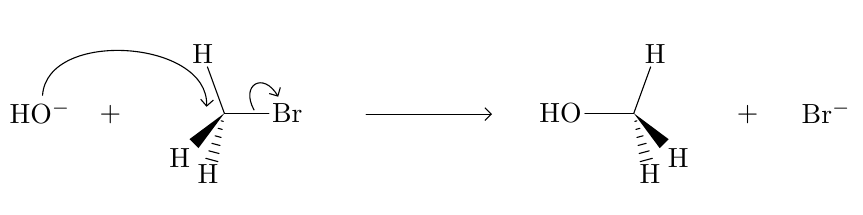
\begin{tikzpicture}[line cap=round, line join=round]
  % atoms
  \node[inner sep=1pt] (a0) at (0,0.762) {\smash{\llap{H}}O\smash{\rlap{$^{-}$}}};
  \coordinate (a1) at (2.326,0.773);
  \node[inner sep=1pt] (a2) at (3.126,0.773) {Br};
  \node[inner sep=1pt] (a3) at (2.052,1.524) {H};
  \node[inner sep=1pt] (a4) at (1.76,0.207) {H};
  \node[inner sep=1pt] (a5) at (2.119,0) {H};
  \coordinate (a6) at (7.526,0.773);
  \node[inner sep=1pt] (a7) at (6.726,0.773) {\smash{\llap{H}}O};
  \node[inner sep=1pt] (a8) at (7.799,1.524) {H};
  \node[inner sep=1pt] (a9) at (8.091,0.207) {H};
  \node[inner sep=1pt] (a10) at (7.733,0) {H};
  \node[inner sep=1pt] (a11) at (9.851,0.762) {Br\smash{\rlap{$^{-}$}}};
  % bonds
  \draw (a1) -- (a2);
  \draw (a1) -- (a3);
  \fill (2.326,0.773) -- (1.997,0.33) -- (1.883,0.444) -- cycle;
  \draw (2.312,0.67) -- (2.286,0.677) (2.299,0.568) -- (2.247,0.582) (2.285,0.466) -- (2.208,0.487) (2.271,0.364) -- (2.168,0.391) (2.258,0.262) -- (2.129,0.296) (2.244,0.159) -- (2.09,0.201);
  \draw (a6) -- (a7);
  \draw (a6) -- (a8);
  \fill (7.526,0.773) -- (7.968,0.444) -- (7.855,0.33) -- cycle;
  \draw (7.565,0.677) -- (7.539,0.67) (7.604,0.582) -- (7.553,0.568) (7.644,0.487) -- (7.566,0.466) (7.683,0.391) -- (7.58,0.364) (7.722,0.296) -- (7.594,0.262) (7.762,0.201) -- (7.607,0.159);
  % pluses
  \node at (0.88,0.762) {$+$};
  \node at (8.971,0.762) {$+$};
  % arrows
  \draw[-{Straight Barb}] (4.126,0.762) -- (5.726,0.762);
  \draw[-{Straight Barb}] (0.017,1.002) .. controls (0.077,1.853) and (2.16,1.706) .. (2.1,0.855);
  \draw[-{Straight Barb}] (2.703,0.815) .. controls (2.523,1.142) and (2.831,1.311) .. (3.01,0.983);
\end{tikzpicture}

\caption{The S$_\mathrm{N}$2 template exported by MecHand to TikZ and compiled
  without modification as part of this article.}
\label{fig:export}
\end{figure}

\subsection{Optional recognition server}

For comparison with image-based recognition, a small FastAPI service wraps DECIMER
(version~2.8.1, hand-drawn model) \cite{Brinkhaus2024}. MecHand sends it a PNG image
of the ink and inserts the structure that DECIMER returns, while arrows and charges
still come from the in-browser recogniser. The server is meant to run on the user's
own computer and is not needed for normal use.

\subsection{Testing, deployment and privacy}

The repository includes unit tests of the recogniser, the recognition benchmark
described below (whose accuracy thresholds act as a regression test), tests of the
KET parser and the exporters, a check that the TikZ and \texttt{chemfig} exports of
every template compile with pdf\LaTeX{}, and end-to-end tests with Playwright in
the Chromium, Firefox and WebKit browser engines. The end-to-end tests open a
template, draw a molecule with the pointer, recognise it, insert it into Ketcher and
export it. One of them uses every feature of the application and fails if any
network request is made after the page has loaded, if any data is sent, or if a
cookie is set; MecHand therefore never transmits the user's drawings or handwriting.
Continuous integration runs all these tests on every change, and the application and
its documentation are deployed as static files to GitHub Pages.

%% ─────────────────────────────────────────────────────────────────────────────
\section{Results and discussion}
\label{sec:results}

\subsection{Recognition of hand-drawn mechanisms}

To measure recognition without a user study, each template was rendered as
synthetic handwriting in three hand styles, which differ in slant, jitter, letter
shapes and in whether arrowheads are drawn with the shaft or as separate strokes
(Figure~\ref{fig:handwriting}). Capital letters were drawn $0.32$ bond lengths tall
and bonds stopped $0.2$ bond lengths short of each label. Each drawing was
recognised and compared with the template after aligning the two by scale and
translation: an atom is correct if its element and charge match, a bond if it joins
the right atoms with the right order, and the arrows if their number and kinds
(electron pair, single electron, reaction) match.

\begin{figure}[t]
\centering
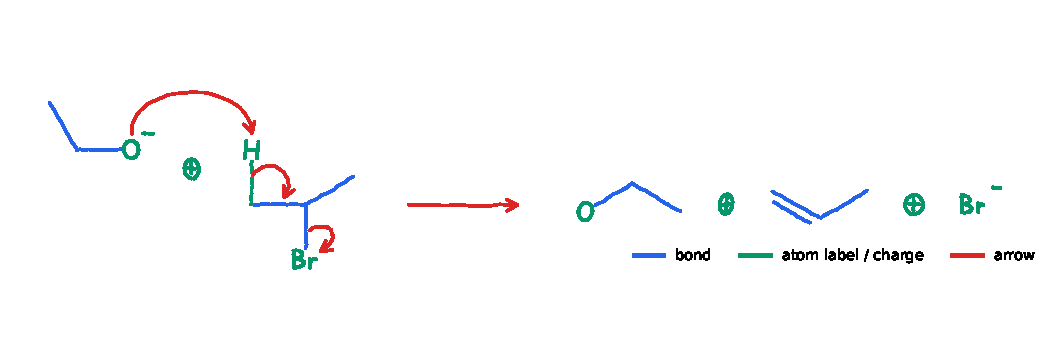
\includegraphics[width=\linewidth]{recognition-e2.pdf}
\caption{Synthetic handwriting of the E2 template, with each stroke coloured by how
  MecHand read it.}
\label{fig:handwriting}
\end{figure}

Over the 39 drawings, MecHand recovered 87\,\% of the atoms, 85\,\% of the bonds and
all of the curved and reaction arrows (Table~\ref{tab:benchmark}); 31\,\% of the
mechanisms were recognised without a single error. The Diels--Alder reaction, the
homolysis of Cl$_2$ and the hydrolysis of SiCl$_4$ were recognised completely. The
main sources of error were crowded metal complexes, where several labels and charge
signs lie close to a metal centre, and labels with many explicit hydrogens.

\begin{table}[t]
\caption{Recognition of synthetic handwriting of the mechanism templates (three hand
  styles per template; percentages of atoms, bonds and arrow sets recognised, and of
  drawings recognised without error).}
\label{tab:benchmark}
\footnotesize
% Generated by manuscript/analysis/make_figures.py — do not edit by hand.
\begin{tabular}{llrrrr}
\toprule
Template & Class & Atoms & Bonds & Arrows & Exact \\
\midrule
SN2 & Org. & 83 & 96 & 100 & 33 \\
E2 & Org. & 96 & 93 & 100 & 33 \\
Nucleophilic addition & Org. & 90 & 86 & 100 & 0 \\
Electrophilic aromatic substitution & Org. & 75 & 76 & 100 & 0 \\
Diels--Alder & Org. & 100 & 100 & 100 & 100 \\
Radical homolysis & Org. & 100 & 100 & 100 & 100 \\
Lewis acid--base adduct & Inorg. & 73 & 71 & 100 & 33 \\
Associative ligand substitution & Inorg. & 70 & 51 & 100 & 0 \\
Hydrolysis of SiCl$_4$ & Inorg. & 100 & 100 & 100 & 67 \\
Brønsted acidity of a metal aqua ion & Inorg. & 75 & 69 & 100 & 33 \\
Serine protease acylation & Biochem. & 89 & 93 & 100 & 0 \\
Alcohol dehydrogenase & Biochem. & 92 & 91 & 100 & 0 \\
Kinase & Biochem. & 90 & 81 & 100 & 0 \\
\midrule
Mean & & 87 & 85 & 100 & 31 \\
\bottomrule
\end{tabular}

\end{table}

\subsection{Comparison with image-based recognition}

To compare with the state of the art for hand-drawn structures, every molecule of
the templates (42 molecules, 126 drawings) was drawn in the same three styles and
read both by MecHand and by DECIMER's hand-drawn model, which received an image of
the same ink. The structures were compared as canonical SMILES with RDKit, after the
same normalisation of every side: explicit hydrogens removed, radicals cleared and
implicit hydrogens recomputed --- so that a label written without its hydrogens is
not counted as an error --- and stereochemistry ignored. Because DECIMER's accuracy
depended on the size of the rendered image, it was run at five scales and its best
result is reported (21--40\,\%).

MecHand returned the exact structure for 65\,\% of the drawings and DECIMER for
40\,\% (Table~\ref{tab:decimer}), with median times of 0.11\,s for MecHand in a
single JavaScript thread and 0.43\,s for DECIMER on a CPU. The comparison is not
neutral: the drawings come from MecHand's own synthetic-handwriting generator, which
was also used while developing the recogniser, and MecHand uses the order and shape
of the strokes, which an image-based model cannot see. It nevertheless shows that,
when the strokes are available --- as they are while the user draws --- a small,
transparent recogniser is competitive with a large deep-learning model, without a
server and in a fraction of the time.

\begin{table}[t]
\caption{Exact recognition (canonical SMILES) of the 126 drawings of the molecules of
  the templates by MecHand and by DECIMER 2.8.1 (hand-drawn model).}
\label{tab:decimer}
% Generated by manuscript/analysis/compare_decimer.py — do not edit by hand.
\begin{tabular}{lrrr}
\toprule
Templates & Drawings & MecHand & DECIMER \\
\midrule
Organic & 48 & 79\,\% & 48\,\% \\
Inorganic & 27 & 48\,\% & 30\,\% \\
Biochemistry & 51 & 61\,\% & 39\,\% \\
\midrule
All & 126 & 65\,\% & 40\,\% \\
\bottomrule
\end{tabular}

\end{table}

\subsection{Export}

The TikZ and \texttt{chemfig} exports of all thirteen templates and of twelve test
structures compile with pdf\LaTeX{}, which is checked automatically. TikZ output
reproduces the layout drawn in Ketcher, including wedges, charges and curved arrows
(Figure~\ref{fig:export}), and is easy to fine-tune by hand because coordinates are
absolute. The \texttt{chemfig} output follows that package's idioms and suits
documents that already use it; its curved arrows are attached to named atoms and
require a second compilation.

\subsection{Comparison with related software}

Table~\ref{tab:features} compares MecHand with related tools. MecHand is the only
one that combines freehand input, recognition of electron-flow arrows and export
to \LaTeX{}; it inherits from Ketcher the editing features of a full structure
editor, including stereochemistry, templates, structure checks and format
conversion. Marvin~JS provides the most complete electron-flow semantics, entered
with toolbar tools, and DECIMER the most capable recognition of hand-drawn
structures from images.

\begin{table}[t]
\caption{Features of MecHand and related software (\yes: available; \no: not available).}
\label{tab:features}
\footnotesize
\begin{tabularx}{\linewidth}{@{}l*{6}{>{\centering\arraybackslash}X}@{}}
\toprule
 & Open source & Runs in browser, no server & Freehand input & Electron-flow arrows & Electron-flow checks & \LaTeX{} export \\
\midrule
MecHand              & \yes & \yes & \yes & \yes & \yes & \yes \\
Ketcher \cite{Karulin2011} & \yes & \yes & \no  & \yes\textsuperscript{a} & \no & \no \\
JSME \cite{Bienfait2013}    & \yes & \yes & \no  & \no  & \no & \no \\
Marvin JS \cite{MarvinJS}  & \no  & \yes & \no  & \yes & \yes & \no \\
ChemInk \cite{Ouyang2011}  & \no  & \no  & \yes & \no  & \no & \no \\
DECIMER \cite{Brinkhaus2024} & \yes & \no & \yes\textsuperscript{b} & \no & \no & \no \\
\bottomrule
\end{tabularx}
\par\smallskip
\raggedright\textsuperscript{a}Elliptical-arc arrows, without attachment to atoms or bonds.
\textsuperscript{b}Images of finished hand drawings (offline recognition).
\end{table}

\subsection{Portability and performance}

MecHand uses only standard web interfaces (Pointer Events, WebAssembly, Web Workers
and SVG) and is tested in the three browser engines that cover current desktop and
tablet browsers. According to MDN's compatibility data \cite{BCD}, all of them
support these interfaces; Safari added coalesced pointer events only in version 18.2,
so older versions record fewer points per stroke without preventing recognition. The
application is about 9\,MB compressed, most of it Ketcher's WebAssembly engine, and
starts in under two seconds from GitHub Pages on a broadband connection.

\subsection{Limitations and future work}

The evaluation uses synthetic handwriting. Real handwriting varies more, which is why
recognition always ends in a confirmation step and why users can teach MecHand their
own writing; a study with students and researchers, recording real pen input, is the
next step%
%% TODO (author): user evaluation with students and researchers (task completion,
%% time, accuracy on real pen input, usability questionnaire), then update this
%% section and the abstract.
. Such recordings would also make it possible to add a trained model of stroke
sequences, for which the recogniser's scene representation and the optional server
already provide the interfaces, and to evaluate on images of mechanisms such as those
in SMiCRM \cite{Leung2024}. Lone pairs are not yet drawn or exported explicitly, and
the electron-flow checker uses simple valence rules rather than full electron
counting.

%% ─────────────────────────────────────────────────────────────────────────────
\section{Conclusions}
\label{sec:conclusions}

MecHand lets chemists and students draw reaction mechanisms by hand, as on paper, and
turns them into editable Ketcher drawings and publication-ready \LaTeX{} code. Its
online recogniser runs in the browser, keeps every drawing on the user's computer,
recognises structures and electron-flow arrows together and checks the electron flow.
On synthetic handwriting it recovers most atoms and bonds and all arrows, and it
recognises hand-drawn molecules more accurately and faster than an image-based
deep-learning model. Because it is built on a standard editor, uses a small and
extensible symbol model, and is tested across browsers, MecHand is easy to adopt in
teaching and research and to extend.

%% ─────────────────────────────────────────────────────────────────────────────
\section{Availability and requirements}

\begin{itemize}
  \item \textbf{Project name:} MecHand
  \item \textbf{Project home page:} \url{https://compbiochbiophlab.github.io/MecHand/}
        (application: \url{https://compbiochbiophlab.github.io/MecHand/app/};
        source code: \url{https://github.com/CompBiochBiophLab/MecHand})
  %% TODO (author): archive the submitted version on Zenodo and add its DOI here.
  \item \textbf{Operating system(s):} Platform independent (web application)
  \item \textbf{Programming language:} TypeScript; Python for the optional
        recognition server and the analysis scripts
  \item \textbf{Other requirements:} A current web browser (Chrome, Edge, Firefox or
        Safari); Node.js~$\geq$\,20.19 to build it; optional Python 3.10--3.13 for the
        DECIMER server
  \item \textbf{License:} MIT (MecHand); Apache~2.0 (Ketcher, used as a dependency)
  \item \textbf{Any restrictions to use by non-academics:} None
\end{itemize}

%% ─────────────────────────────────────────────────────────────────────────────
\section*{Abbreviations}
CDXML: ChemDraw XML; KET: Ketcher JSON format; MDL: MDL molfile and reaction file
formats; OCSR: optical chemical structure recognition; SMILES: simplified molecular
input line entry system; WASM: WebAssembly.

\backmatter

\bmhead{Availability of data and materials}
The source code, the mechanism templates, the synthetic-handwriting benchmark, the
comparison dataset and the scripts that produce every table and figure of this article
are available at \url{https://github.com/CompBiochBiophLab/MecHand}
(\texttt{manuscript/analysis/}).

\bmhead{Competing interests}
The author declares that he has no competing interests.

\bmhead{Funding}
%% TODO (author)
Not applicable.

\bmhead{Authors' contributions}
%% TODO (author): CRediT roles.
JVF conceived and developed MecHand, performed the analyses and wrote the manuscript.

\bmhead{Acknowledgements}
%% TODO (author)
The author thanks the developers of Ketcher, Indigo, RDKit and DECIMER for making
their software openly available.

%% TODO (author): Springer Nature's editorial policy requires that the use of large
%% language models or other generative AI tools for writing text or code be described
%% (e.g. in the Implementation/Methods section or the Acknowledgements); AI-assisted
%% copy editing of the author's own text does not need to be declared. Add the
%% required statement here before submission.

%% ── References ───────────────────────────────────────────────────────────────
%% The style comes from the sn-jnl class option (sn-vancouver-num); do not add
%% \bibliographystyle here.
\bibliography{references}

\end{document}
